\documentclass{bioinfo}
\copyrightyear{2018} \pubyear{2018}
\usepackage{natbib}
\usepackage[hidelinks]{hyperref}
\setcitestyle{round, author-year}

\access{Advance Access Publication Date: Day Month Year}
\appnotes{Original Paper}

\newcommand{\raxml}{RAxML}
\newcommand{\eggnog}{EggNOGG}
\newcommand{\epa}{EPA-ng}
\newcommand{\papara}{PaPaRa}
\newcommand{\phyma}{PhyloMagnet}

\begin{document}
\firstpage{1}

\subtitle{Sequence analysis}

\title[PhyloMagnet]{PhyloMagnet: Fast and accurate profiling of short-read meta-omics data using gene-centric phylogenetics}
\author[Sch\"on et al.]{Max E. Sch\"on\,$^{\text{\sfb 1,}*}$, Laura Eme\,$^{\text{\sfb 1}}$, Thijs J.G. Ettema\,$^{\text{\sfb 1,2,}*}$}
\address{$^{\text{\sf 1}}$Department of Cell and Molecular Biology, Science for Life Laboratory, Uppsala University, SE-75123 Uppsala, Sweden, $^{\text{\sf 2}}$Laboratory of Microbiology, Department of Agrotechnology and Food Sciences, Wageningen University, Stippeneng 4, 6708WE Wageningen, The Netherlands}


\corresp{$^\ast$To whom correspondence should be addressed.}

\history{Received on XXXXX; revised on XXXXX; accepted on XXXXX}

\editor{Associate Editor: XXXXXXX}

\abstract{\textbf{Motivation:}Metagenomic and metatranscriptomic sequencing analyses have become increasingly popular tools for  producing massive amounts of short-read data, often used for the reconstruction of draft genomes or the detection of (active) genes in microbial communities. Unfortunately, sequence assemblies of such datasets generally remain a computationally challenging task. Frequently, researchers are only interested in a specific group of organisms or genes; yet, the assembly of multiple datasets only to identify candidate sequences for a specific question is prohibitively slow, forcing researchers to select a subset of datasets to address their question (e.g. based on prior knowledge on the possible presence of the organism/gene). Here we present PhyloMagnet, an approach to screen meta-omics datasets for taxa and genes of interest using gene-centric assembly and phylogenetic placement of sequences.\\
\textbf{Results:} Using PhyloMagnet, we could identify up to 87\% of the genera in an in-vitro mock community with variable abundances, while the false positive predictions per single gene tree ranged from 0\% to 23\%. When applied to a group of metagenomes for which a set of MAGs have been published, we could detect the majority of the taxonomic labels that the MAGs had been annotated with. In a metatranscriptomic setting the phylogenetic placement of assembled contigs corresponds to that of transcripts obtained from transcriptome assembly.\\
\textbf{Availability:} PhyloMagnet is built using Nextflow, available at \href{https://github.com/maxemil/PhyloMagnet}{github.com/maxemil/PhyloMagnet} and is developed and tested on Linux. It is released under the open source GNU GPL license and documentation is available at \href{https://phylomagnet.readthedocs.io/en/latest/}{phylomagnet.readthedocs.io}.\\
\textbf{Contact:} \{max-emil.schon;thijs.ettema\}@icm.uu.se\\
\textbf{Supplementary information:} Supplementary data are available at \textit{Bioinformatics}
online.}

\maketitle

\section{Introduction}
High-throughput DNA sequencing has revolutionized biology, opening up new fields of research and enabling new insights. There are several sequencing technologies available, each having different technological advantages and limitations and differing significantly in sequence read length, quality and throughput. Still leading the market is Illumina’s short read platform, which offers the lowest per base cost and error rate as well as a tremendous output (Mitchell et al. 2017, Mardis 2017). Rather recent applications comprise DNA shotgun sequencing as well as RNA sequencing of complex microbial communities, termed metagenomics and metatranscriptomics, respectively. 

Using genome-resolved or genome-centric metagenomics, genomes of previously uncultured species can be extracted in large quantities from shotgun metagenomic sequencing data of microbial communities. Large environmental sequencing initiatives like the Tara Oceans project (Sunagawa et al. 2015) have provided researchers with enormous amounts of metagenome data. Metagenomic binning algorithms to reconstruct genomes from metagenome assemblies have been developed and improved at a fast rate. Together with the ever increasing sequencing capacity however, it becomes harder to decide which of the available samples (publicly available or specifically sequenced for your study) actually contain sequence data from the taxon of interest. This is due to the rather compute intense metagenome assembly which needs to be performed in order to apply genome binning tools.

Instead of assembling short reads into longer contigs, the taxonomic composition of a metagenomic or metatranscriptomic sample, microbiome profilers that classify reads can be used. There is a plethora of tools available that assign reads to a reference taxonomy. They generally base their classification on the alignment of reads to references, similar to the blast algorithm (Megan, Metaphlan) or use exact k-mer matches to classify reads (Clark, Kraken). Development in this area is continuing in order to be able to increase analysis speed while reducing the memory footprint. Currently diamond is one of fastest local aligners that has sensitivity comparable to blast, and MetaCache is one of the fastest and most memory efficient k-mer based classifiers, using the MinHash technique. Both of these approaches, however, are based on sequence similarity, which can be incongruent with the true phylogenetic relationship of sequences (Smith and Pease, 2016).

Traditional phylogenetic tools on the other hand offer several robust evolutionary models for both nucleic and amino acids, but are slow compared to similarity based methods, usually prohibiting their application to whole metagenome samples. A major issue is also that short reads usually do not provide enough phylogenetic signal, leading to artifactual inferences (Madsen et al. 2011). Several tools have been developed to overcome these barriers by instead placing fragmentary sequences (particularly from amplicon sequencing data) onto a phylogenetic reference tree (Madsen et al. 2011, Berger et al. 2011, Barbera et al. 2018).

Gene-centric analyses of metagenomic and metatranscriptomic data partitions the short reads or the assembled sequences by their affiliation to genes or gene families. These methods can be used to see what genes are present or active in a sample, and can be combined with assemblers to reconstruct full-length sequences for a gene of interest. MATAM is a gene-centric targeted assembler that aims to reconstruct full-length sequences via an overlap graph of candidate reads, but currently is limited to the 16S rRNA gene. In contrast, the MEGAN assembler recontructs contigs based on the alignment of reads to (arbitrary) reference protein sequences (Huson et al. 2016).

A recently published tool, GraftM, uses the ideas of phylogenetic placement and gene-centric metagenomic to taxonomically classify sequences of genes within metagenomes. It is capable of placing either short read sequences or assembled metagenomes onto a reference tree, but does not employ a gene-centric assembler.

The goals of this study were to create a computational workflow that 
\begin{enumerate}
\item could determine the presence of taxa of interest in large short read samples based on gene-centric assembly and robust phylogenetic inference, especially with the objective of selecting good candidate samples for metagenomic assembly and genome-resolved metagenomics.
\item The workflow should use state-of-the-art methods and be versatile and fast enough to accommodate a broad range of applications while being modular in order to easily incorporate new approaches.
\item We compared the workflow’s performance in terms of computational footprint and sensitivity/specificity to GraftM, another recently published tool with a similar application.
\end{enumerate}


\begin{methods}
\section{Implementation}
PhyloMagnet uses the idea of gene-centric assembly (Huson et al. 2017) to efficiently screen samples of short reads for target genes. Below is a description of the analysis steps employed by the pipeline. 

\begin{figure*}[!tpb]%figure1
\centerline{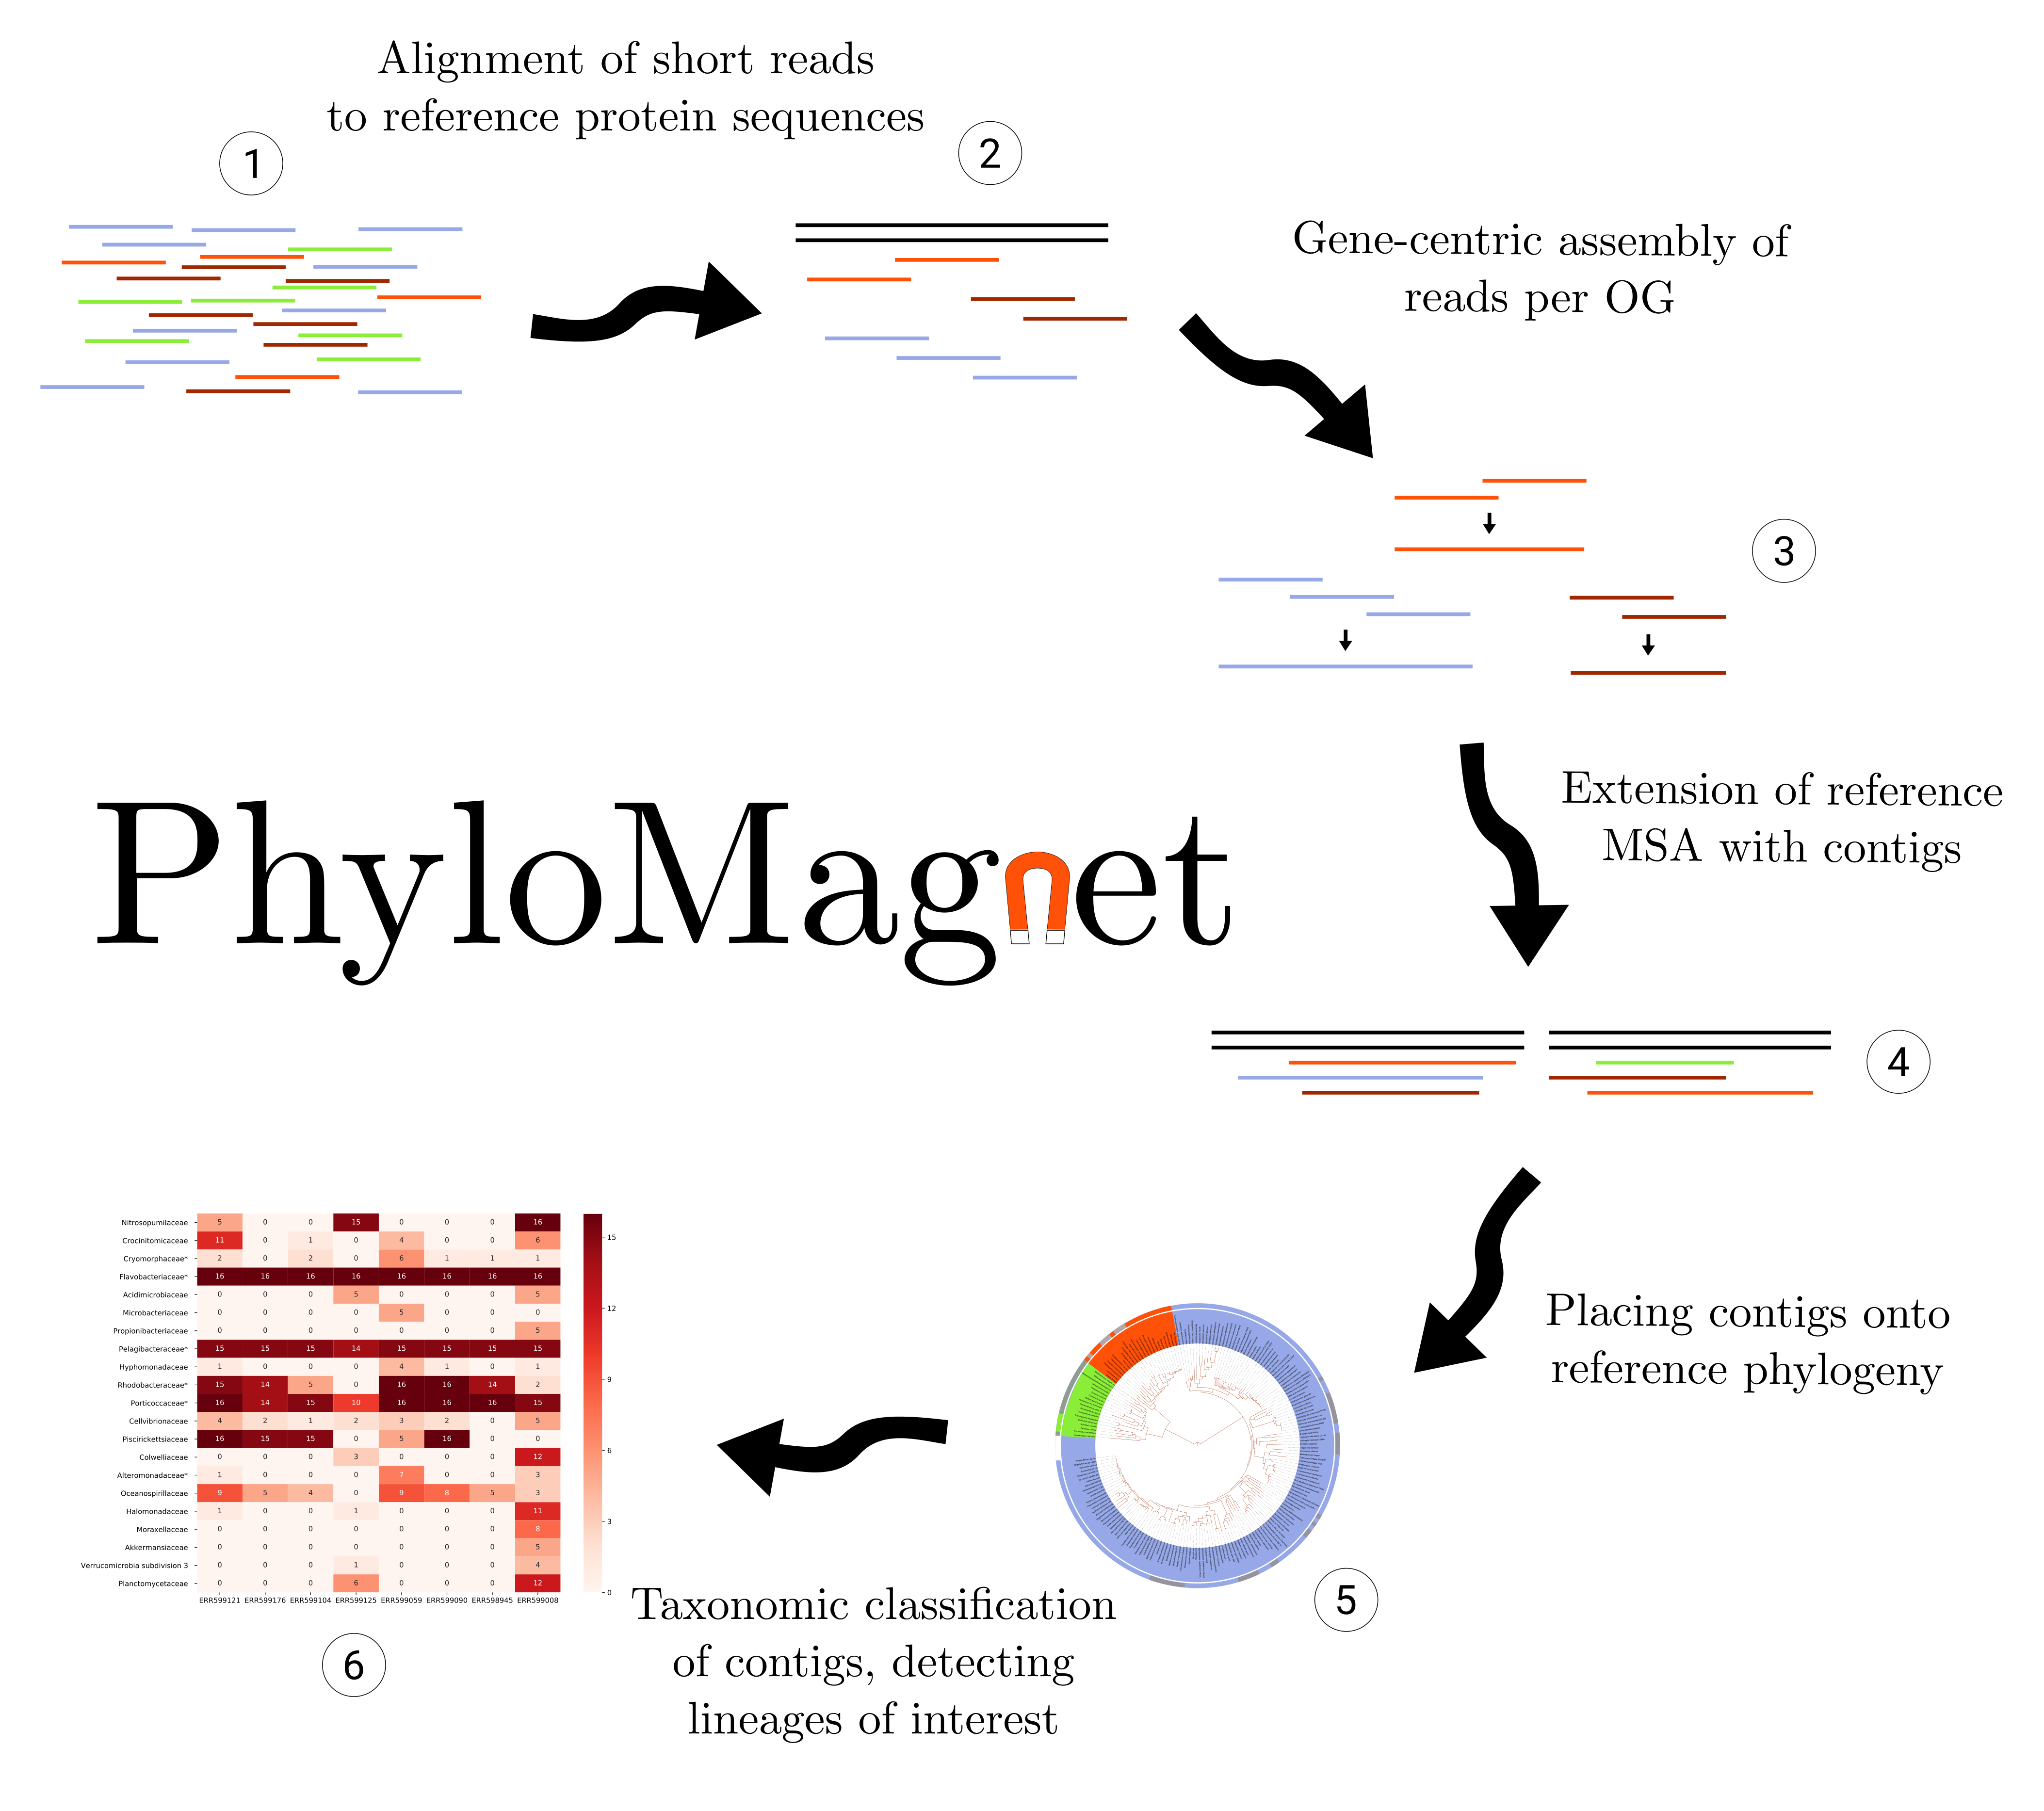
\includegraphics[width=\textwidth]{figures/Fig1.png}}
\caption{Caption, caption.}\label{fig:01}
\end{figure*}

\subsection{Alignment to reference protein sequences}
As (orthologous) groups of reference proteins either EggNOG identifiers can be specified or a set of sequences curated by the user in fastA format can be given as input []. Each of the short read samples given as input is aligned to the whole collection of reference protein sequences using diamond in blastX mode (Buchfink et al. 2015).
\subsection{Gene Centric Assembly of reads}
Using the gene-centric assembler implemented in MEGAN (Huson et al. 2016, 2017), contigs of nucleotide sequences  belonging to each reference group are assembled and subsequently translated into amino acid sequences.
\subsection{Alignment and tree reconstruction of reference}
Each group of reference sequences is aligned using either mafft or prank, and a reference tree is reconstructed using any of iqtree, raxml of fasttree, making it possible to choose the appropriate method for a specific analysis. This way the user can weigh out speed vs. quality of the reference tree. Reference alignment and tree can also be precomputed (e.g. on a local machine) and then provided to PhyloMagnet as a reference package (e.g. on a computing cluster or by a collaborator). 
\subsection{Placement of reconstructed protein sequences}
The alignments of each reference group are extended with the assembled contigs using papara [], preserving the previously computed reference alignment. This extended alignment is then used to place contigs onto the reference tree using the evolutionary placement algorithm (\epa). Finally, the placement results are analysed using gappa, and a summary of taxonomic labels is produced.
\subsection{'Magnetizing' and decision on relevance}
Based on the occurrence of taxonomic labels per sample in each reference group, a decision is made whether the sample is a good candidate to contain sequences (genomes or transcripts) of a certain taxonomic group. Several summary tables and plots are produced to help the manual inspection of the results. 
\subsection{Availability}
PhyloMagnet is written as a nextflow pipeline and available on github (github.com/maxemil/PhyloMagnet). Several functions and utilities are implemented either in python or bash. All needed dependencies are available as a singularity image (singularity-hub.org/collections/978) and the documentation can be found on ReadTheDocs (phylomagnet.readthedocs.io).
\section{Benchmarking}
To evaluate the performance of our workflow and exemplify its potential uses, we performed three benchmark experiments using an in vitro mock community as well as environmental metagenomic and metatranscriptomic sequencing datasets. We chose the datasets such that we could compare the results produced by PhyloMagnet to reference genome mapping data \citep{Singer2016}, genomes extracted from metagenomes with taxonomic annotation \citep{Delmont2018} and an assembled metatranscriptome \citep{Frazier2017}, respectively. For details on command line parameters see the supplementary methods.

\subsection{Reference sequences}
To assess the general taxonomic composition of datasets we used a set of 16 ribosomal proteins (rp16) that are thought to represent reliable phylogenetic markers, as they should be vertically inherited throughout the evolution of life and present in a single copy in most organisms (Brown et al. 2015). For this, we downloaded the corresponding sets of unaligned homologous sequences from the \eggnog\ database v4.5.1 \cite[][see Table SXXX]{huerta-cepas_eggnog_2016}.

As a second set of reference protein sequences, we used the set of 12 protein coding genes known to be present in chloroplast genomes of Dinophyceae (Howe et al. 2007). This phylum of single-celled algae can be found in a wide range of aquatic environment and notably contains coral symbionts within the genus \textit{Symbiodinium} []. For each of the genes we downloaded all available curated chloroplast encoded protein sequences for all phyla from uniprot (Apweiler et al. 2004) as well as all available proteins from the Dinophyceae from the same database.

\subsection{Data sets}
The first dataset we selected was the MBARC-26 (Mock Bacteria ARchaea Community), a mock community of 23 bacterial and 3 archaeal strains with finished reference genomes that were pooled and sequenced on an Illumina HiSeq instrument []. To test whether we could retrieve all organisms, we added orthologous sequences to the rp16 references for those genera missing from EggNOG. We used available genomes from related species within the same genera and selected the orthologous proteins by performing a HMM search against the proteomes. These extended rp16 references were then used to analyse the MBARC-26 short read data. 

As a second data set we used samples from the TARA Oceans Initiative, restricted to those samples defined as Southern Ocean by Delmon et al. 2018. We used the rp16 references to assess taxonomic composition in those samples and compared the results to the taxonomic classification of the MAGs recovered by Delmont et al.

Finally, we used the Dinophyceae chloroplast references to search for Dinophyceae (especially Symbiodinium) sequences in the Metatranscriptome published by [] and compared the assembled sequences and their placement in the reference tree with the sequences from the metatranscriptomic assembly available at [].

\subsection{Comparison with GraftM}
We compared the performance of PhyloMagnet with that of the recently published tool GraftM. GraftM also places sequences (either unassembled reads or pre-assembled contigs) onto a reference phylogeny using the tool pplacer, for which \epa\ represents a scalable replacement that is able to handle larger amounts of data.

We created GraftM reference packages (gpkgs; containing the reference alignment, tree and the taxonomic annotation) from each of the extended rp16 references using the create command (see supplementary methods). We then used each gpkg to analyse the MBARC-26 dataset and recovered taxonomic classifications of the query sequences.
For both tools, we counted the number of genera that were correctly identified in each tree (true positives) as well as the number of genera that were identified even though they were not present in the MBARC-26 mock community (false positives). We also assessed the runtime and memory consumption of both tools for analysis of the full MBARC-26 dataset (50 Gb) as well as for subsamples of 1\% and 10\% (0.5 and 5\,Gb, respectively).

\end{methods}

\section{Results}
\subsection{MBARC-26}
We evaluated the performance of PhyloMagnet and GraftM to detect the presence of the 24 MBARC genera (23 of those detectable, as Nocardiopsis was not sequenced in Singer et al. 2016) in the metagenomic sample (Fig S1 and Table S1). The number of correctly detected as well as falsely reported genera are displayed in Fig 2. PhyloMagnet reported up to 20 of the MBARC genera and around 2 (up to 7) false positive genera in all of the 16 trees. In contrast, GraftM identified a maximum of 9 of the correct MBARC genera while giving around 4 (up to 14) false positives for each tree. Some of the reported errors could be attributed to closely related and possibly unresolved taxonomic groups such as Meiothermus/Thermus and Escherichia/Salmonella. Several Taxa with very low abundance in the data (e.g. Corynebacterium and Clostridium) were picked up by GraftM but not PhyloMagnet, which is likely due to the fact that there are not enough reads to reconstruct longer contigs for theses taxa, impeding an identification by PhyloMagnet.
When comparing results for the full dataset and the subsampled datasets, PhyloMagnet seems to profit immensely from the additional data, likely because the assembler can connect more reads and thus reconstruct more contigs above the length threshold.
In terms of runtime, PhyloMagnet provides a twofold speedup over GraftM on 10 CPUs, making more efficient use of available computational resources, whereas consuming significantly more memory (due to the high memory requirements of MEGAN, see Fig S1).
There seems to be a correspondence, although not proportional, between the percentage of mapped reads in Singer et al. 2016 and the number of trees a genus was detected in (Fig S2). Clearly there is also an issue with taxa where phylogeny and taxonomy disagree such as for the Salmonella/Escherichia group.

\begin{figure*}[!tpb]%figure1
\centerline{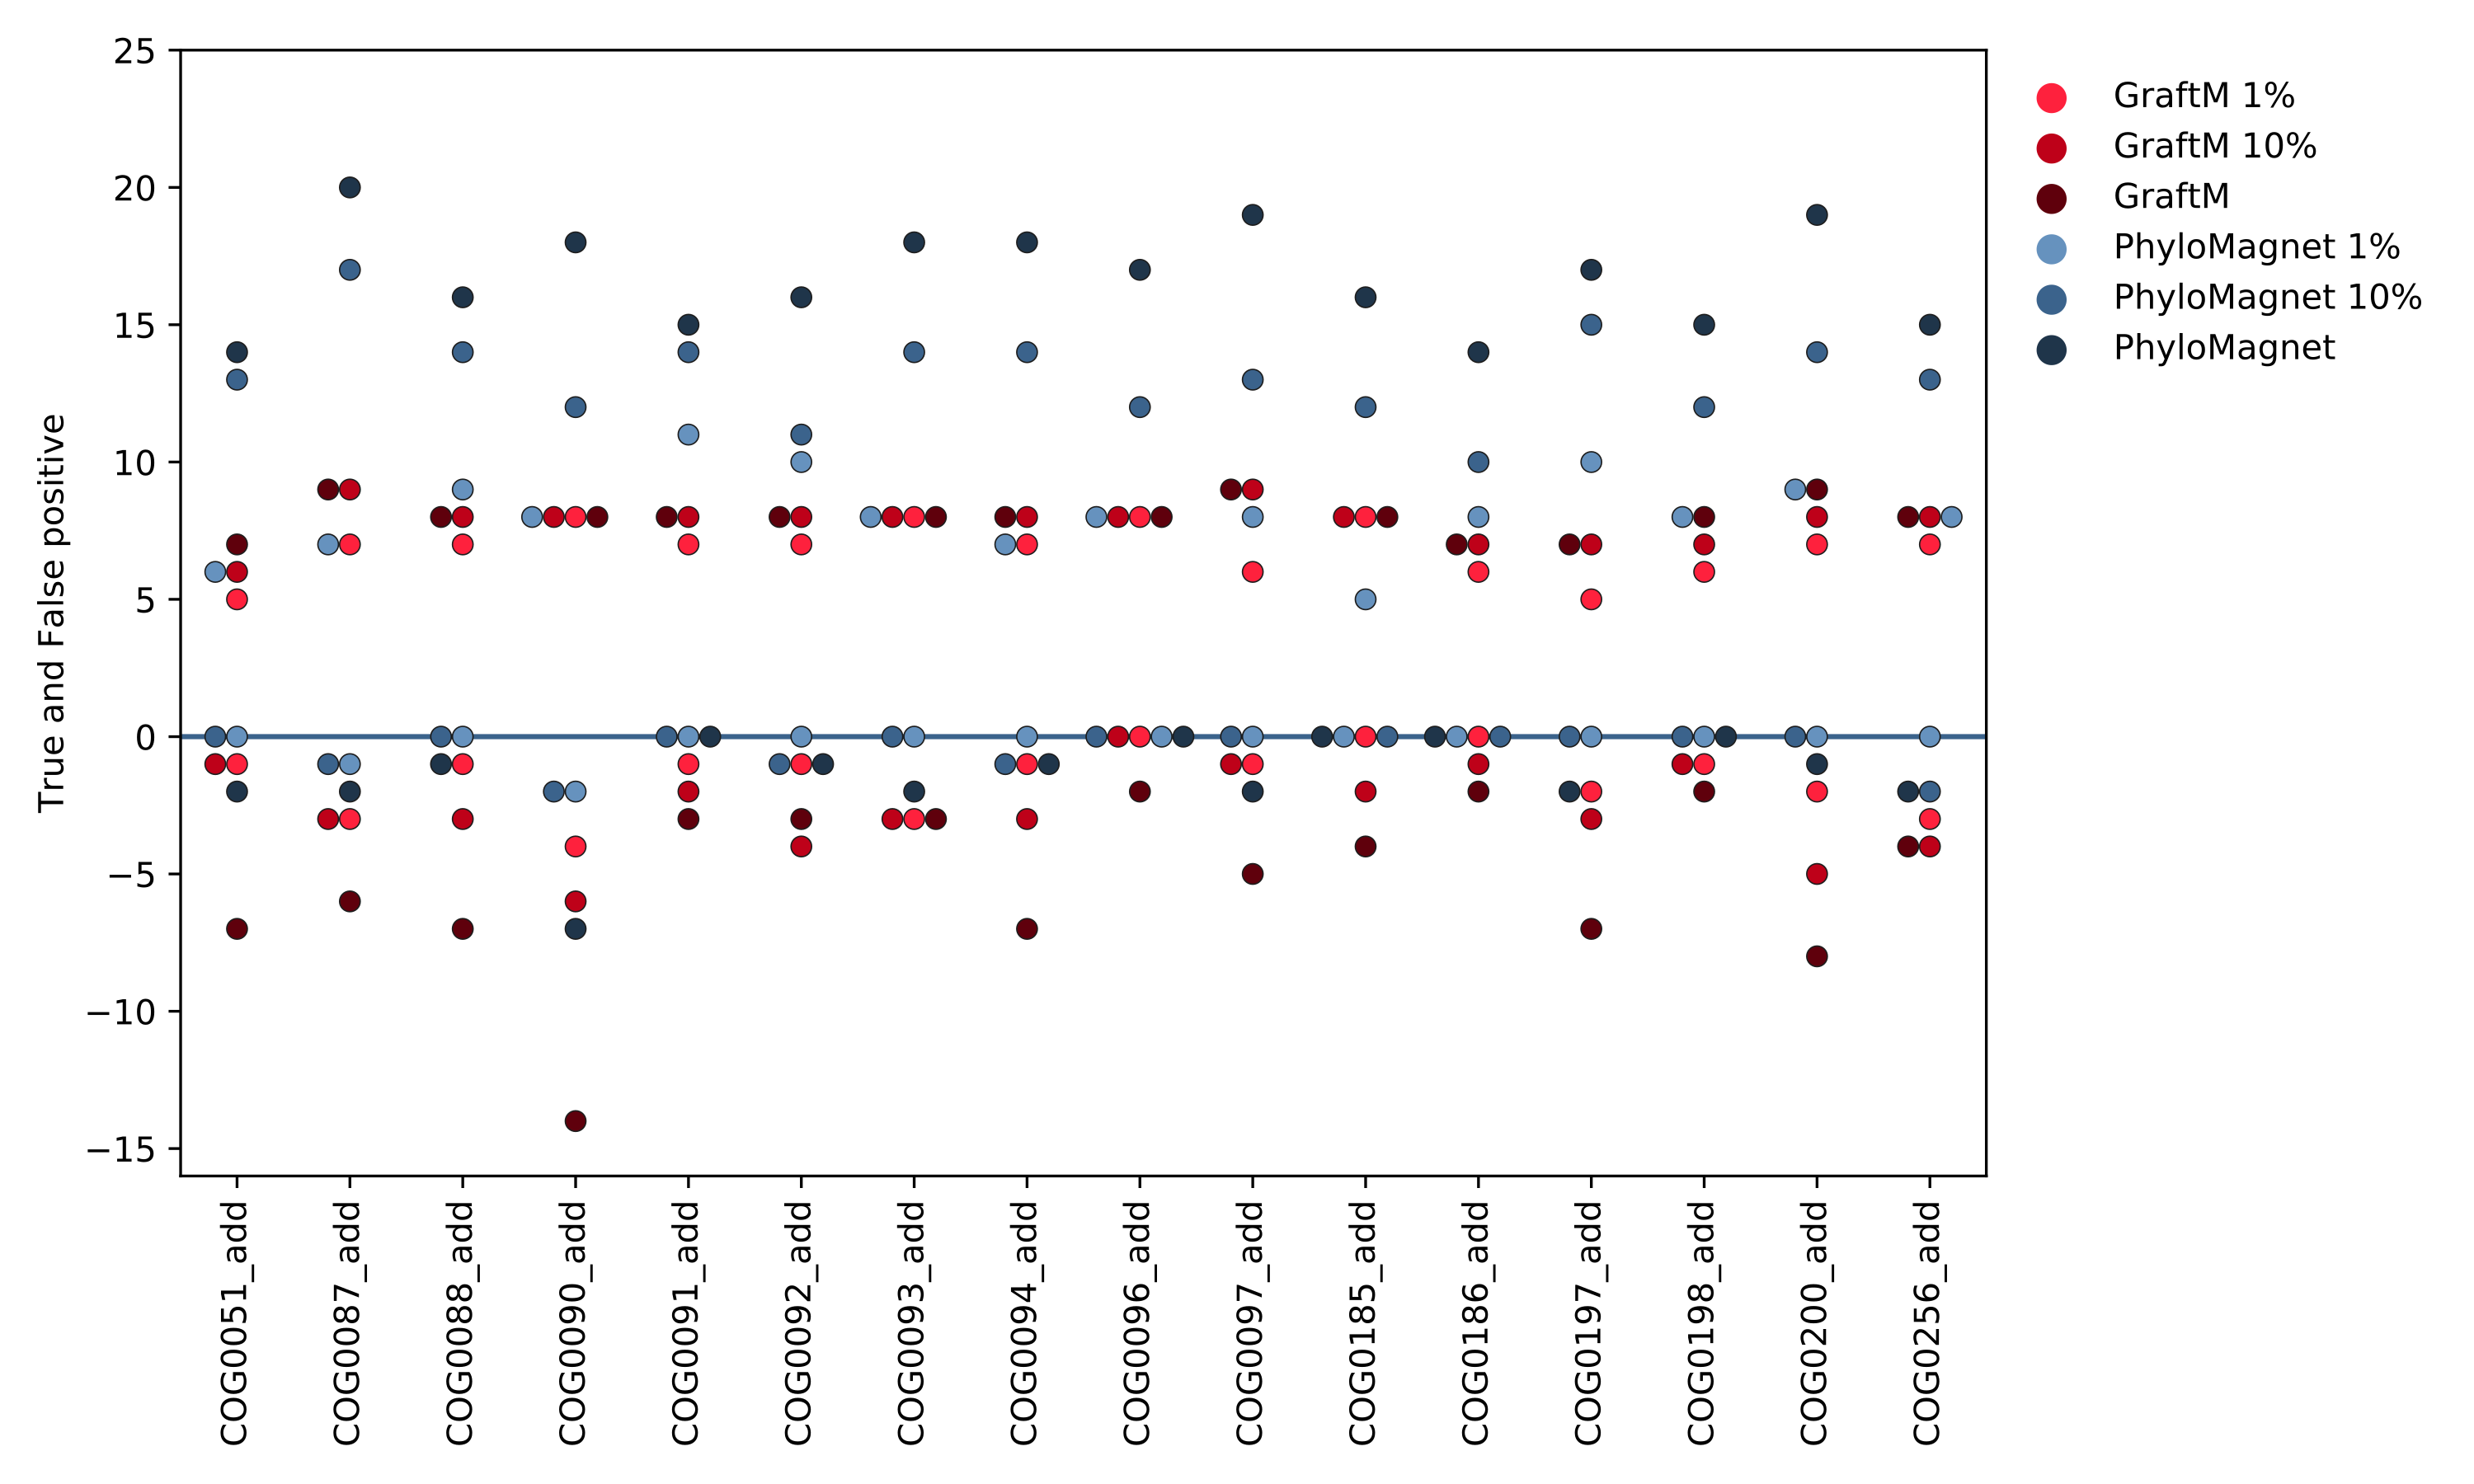
\includegraphics[width=\textwidth]{figures/Fig2.png}}
\caption{Caption, caption.}\label{fig:02}
\end{figure*}

\subsection{TARA Southern Ocean}
As shown in Fig 3, genes classified as belonging to genomes of the Flavobacteriaceae were detected in all samples and trees, reflecting the results from Delmont et al. 2018, who recovered 6 non-redundant MAGs within the Flavobacteriales. We marked all those families that were recovered by Delmont et al. in Fig 3. These include one MAG each from the Alteromonadaceae, the Rickettsiales and the Alphaproteobacteria as well as two Gammaproteobacteria. All of these can be found in our results except for the Rickettsiales, who could be confounded with the Pelagibacterales because of common streamlining in their genomes, an issue known to cause phylogenetic artifacts (Roger et al. 2017). It is very likely that the MAGs/Bins that are labelled as Gammaproteobacteria are members of the Piscirickettsiaceae or Porticoccaceae, which were both detected in several individual samples and the majority of single gene trees. Additional taxonomic labels that could be assigned to raw genomic bins from the same study (Tab S2) yielded additional taxonomic labels recovered in our gene-centric analysis (Porticoccaceae, Rhodobacteraceae, Pelagibacteraceae, Cryomorphaceae). Some of the labels we recovered were not represented by genomic bins, indicating either false positive classification of contigs or a low abundance of the genomic DNA, such that no genome bins could be reconstructed.

\begin{figure*}[!tpb]%figure1
\centerline{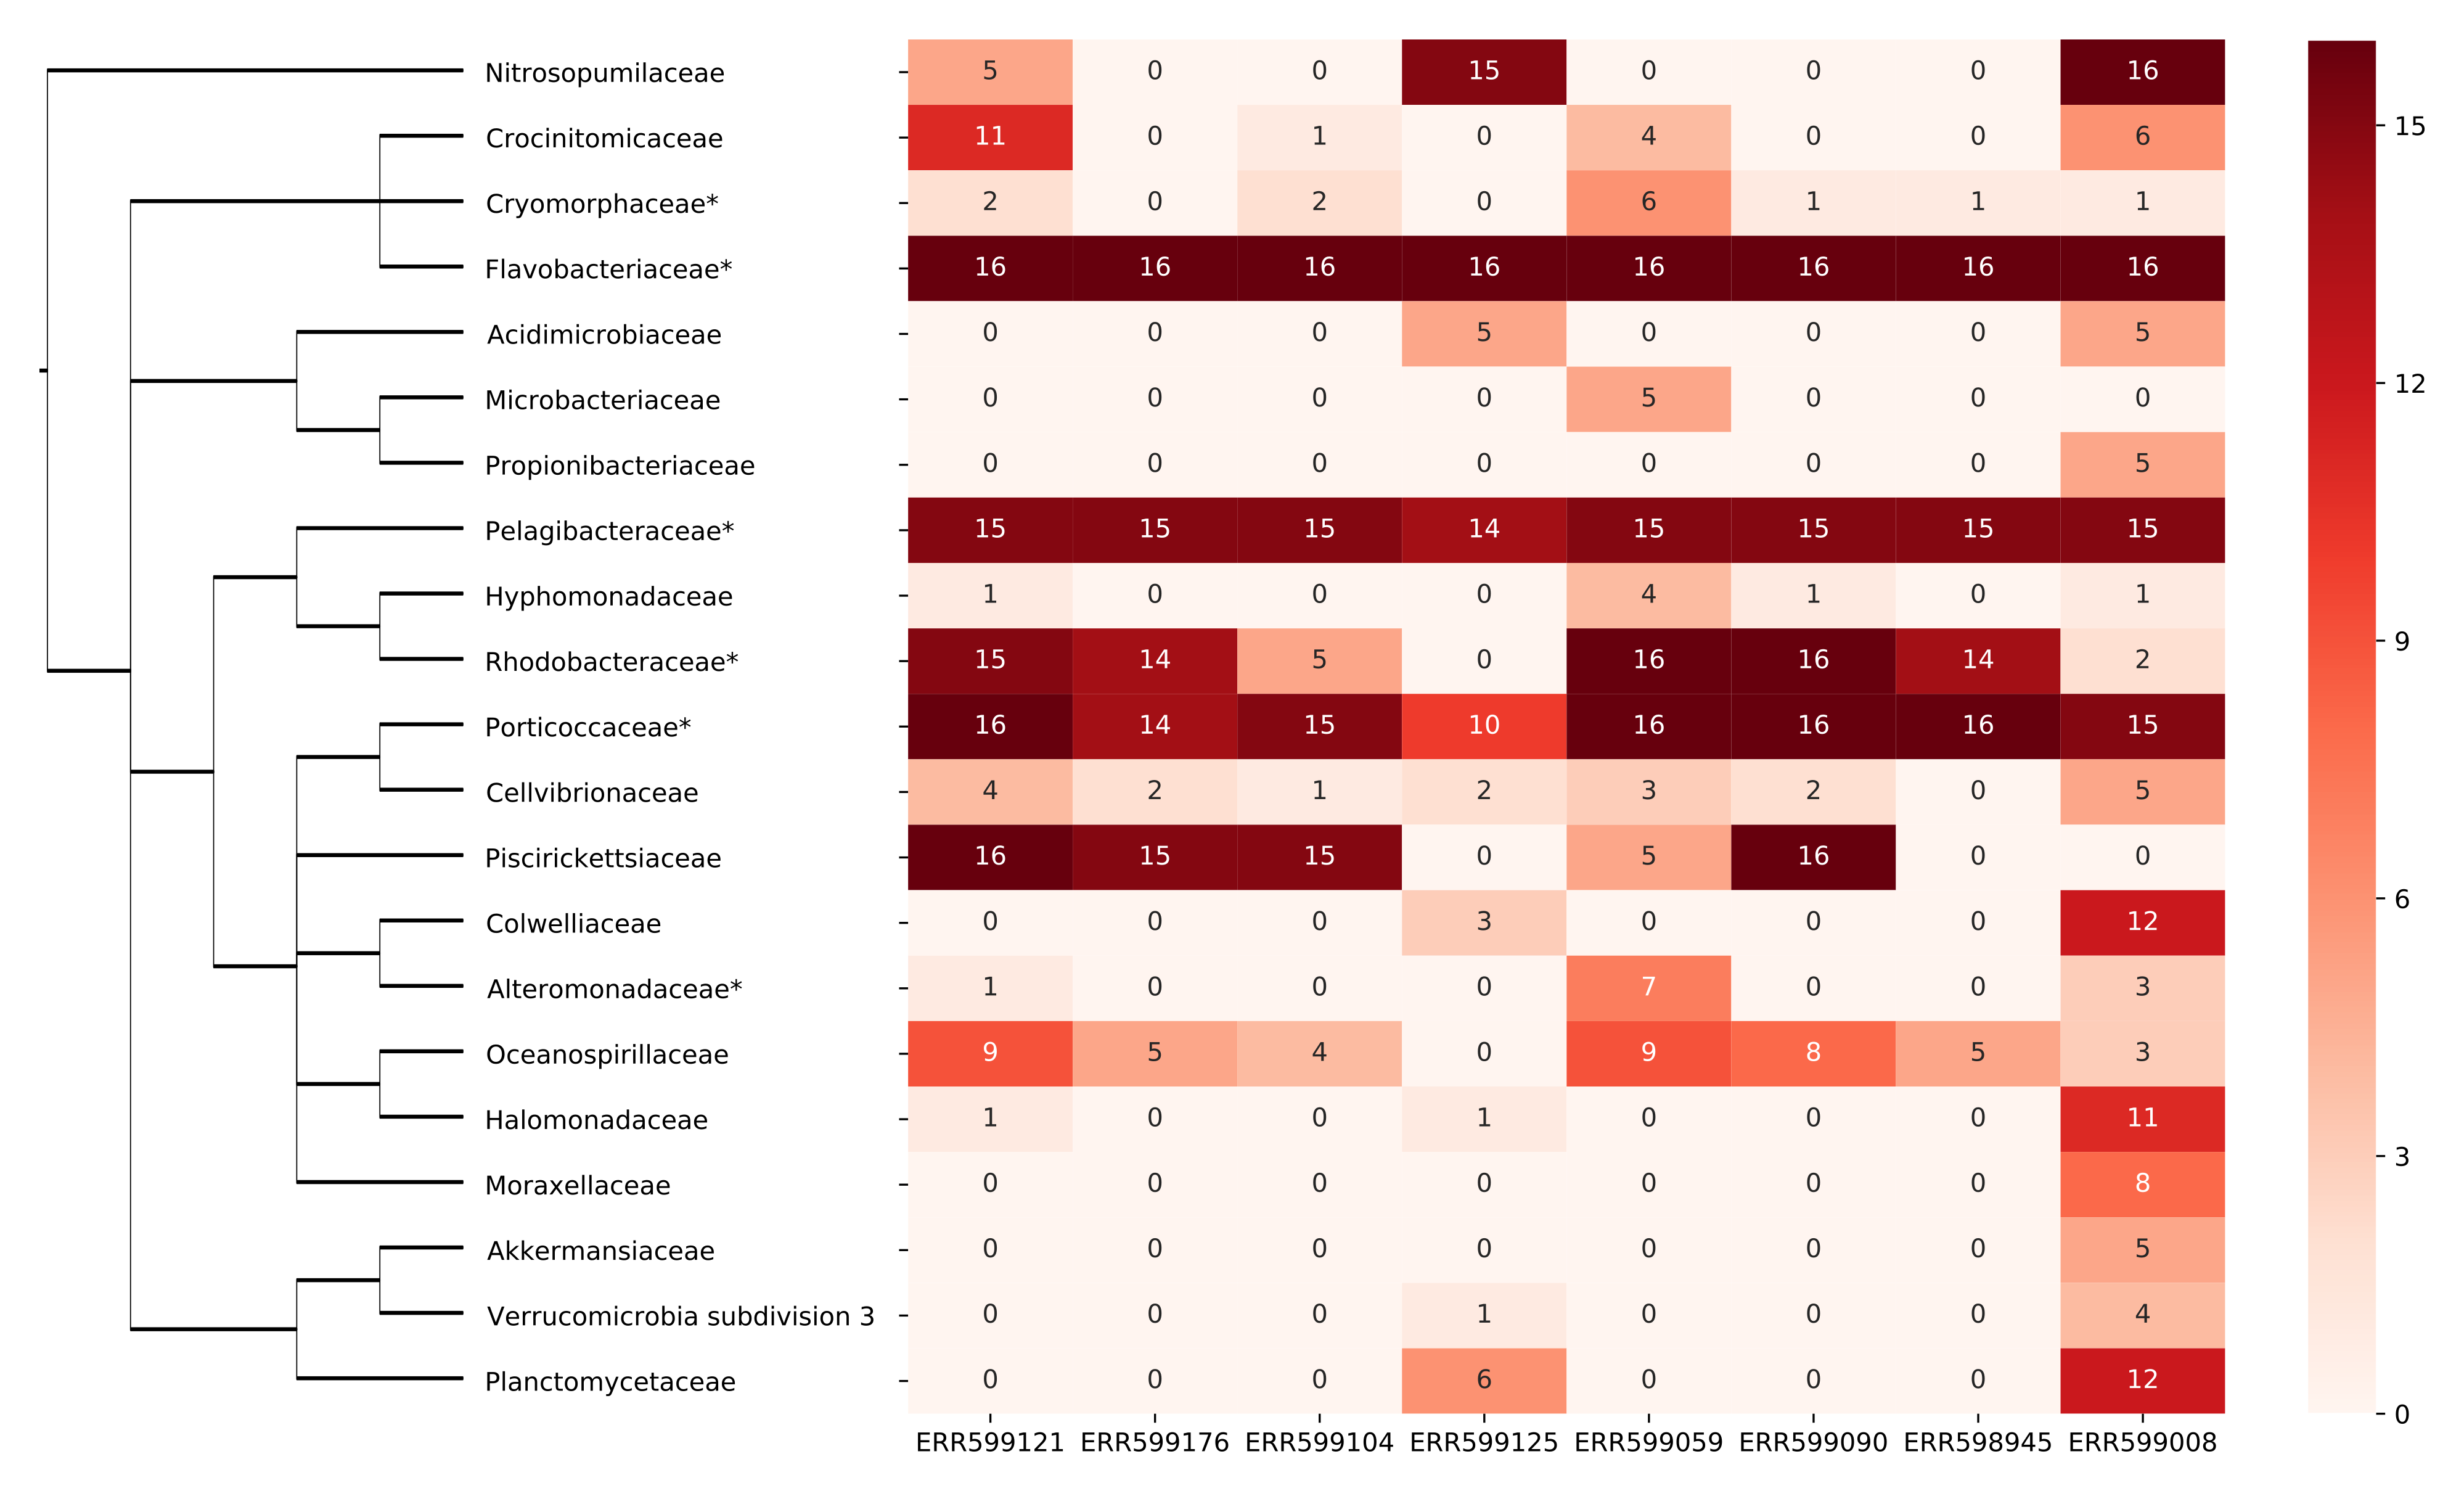
\includegraphics[width=\textwidth]{figures/Fig3.png}}
\caption{Caption, caption.}\label{fig:03}
\end{figure*}

\subsection{Coral Bleaching}
Contigs classified as Symbiodiniaceae could be identified in 10 out of the 12 chloroplast gene reference trees. The number of contigs we reconstructed from the pooled sequencing data of 23 samples ranged from 2 (psbE) to as many as 169 (psbA), whereas we could identify either 1 or 2 transcripts from the assembled transcriptome for 9 out of the 12 genes. The two genes for which no contigs could be reconstructed were psbI and petD, both missing in the assembled transcriptome as well, likely because of two dissimilar restraints. The psbI gene is only around 30aa long, making contigs shorter than the minimum length of 200bp. Additionally it has, within the Dinophyceae, only been identified in the species Amphidinium operculatum, and not in Symbiodinium (Nisbet et al. 2004, Barbrook et al. 2014). As for petD, it seems that its transcription level is quite low, so that very few reads would have been sequenced, making assembly of contigs or transcriptomes virtually impossible (Nisbet et al. 2008). In those cases where transcripts could be identified, they were generally placed on the same branches or very close ones within the reference tree as were all of the corresponding contigs (Fig 4).

\section{Discussion}


\section{Conclusion}


\section*{Acknowledgements}

\section*{Funding}
MES is funded by the Horizon 2020 research and innovation program under the Marie Sk\l{}odowska-Curie ITN project SINGEK (http://www.singek.eu/; grant agreement No. H2020-MSCA-ITN-2015-675752).

%\bibliographystyle{natbib}
\bibliographystyle{bioinformatics}
\bibliography{PM.bib}

\end{document}
